\documentclass[10pt,a4paper,oneside]{article}
\usepackage{amsmath,amsthm,amssymb,floatrow}
\usepackage{lmodern}
\usepackage{geometry}
\usepackage{graphicx,float,subfigure,ctex}
\DeclareGraphicsExtensions{.pdf,.jpeg,.png,.jpg}
\geometry{left=2.18cm,right=2.18cm,top=1.54cm,bottom=2.0cm}
\pagestyle{empty}
\title{\bf 运筹学实验报告-1}
\author{姓名:李奕萱  学号:PB22000161 }
\date{\today}

\begin{document}

\maketitle

\section{问题背景}

线性规划(Linear Programming,简称LP)作为运筹学的核心工具之一,
旨在通过线性方程和不等式的约束条件,寻找一个最优的决策方案。线性
规划问题的求解方法包括单纯形法、对偶单纯形法、内点法等,其中单纯
形法是应用最广泛的算法之一。

然而,在实际问题中,线性规划往往伴随有特殊情况,如无可行解、无界
解或冗余约束等,这些情况可能使得问题求解过程更加复杂。因此,在求
解线性规划时,如何高效处理这些特殊情况并获得最优解,是运筹学中的
一个重要课题。

本实验旨在通过单纯形法这种常见算法来求解线性规划问题,并
通过实验验证这种算法的有效性、稳定性和计算效率。

\section{算法介绍}

\subsection{前期准备}

\begin{figure}[H]
    \centering
    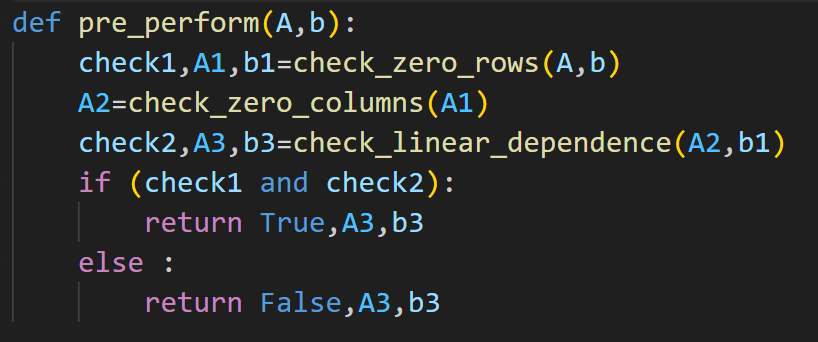
\includegraphics[width=0.6\textwidth]{屏幕截图 2024-11-05 104451.png}
\end{figure}

在进行线性规划求解之前,需要进行一些前期处理工作。
首先,我们检查输入的矩阵是否存在全零行、全零列以及
简单的线性相关行。如果有这些问题,需将对应的行或列
删除,以简化问题的求解过程。

\subsection{转化为标准形式}

\begin{figure}[H]
    \centering
    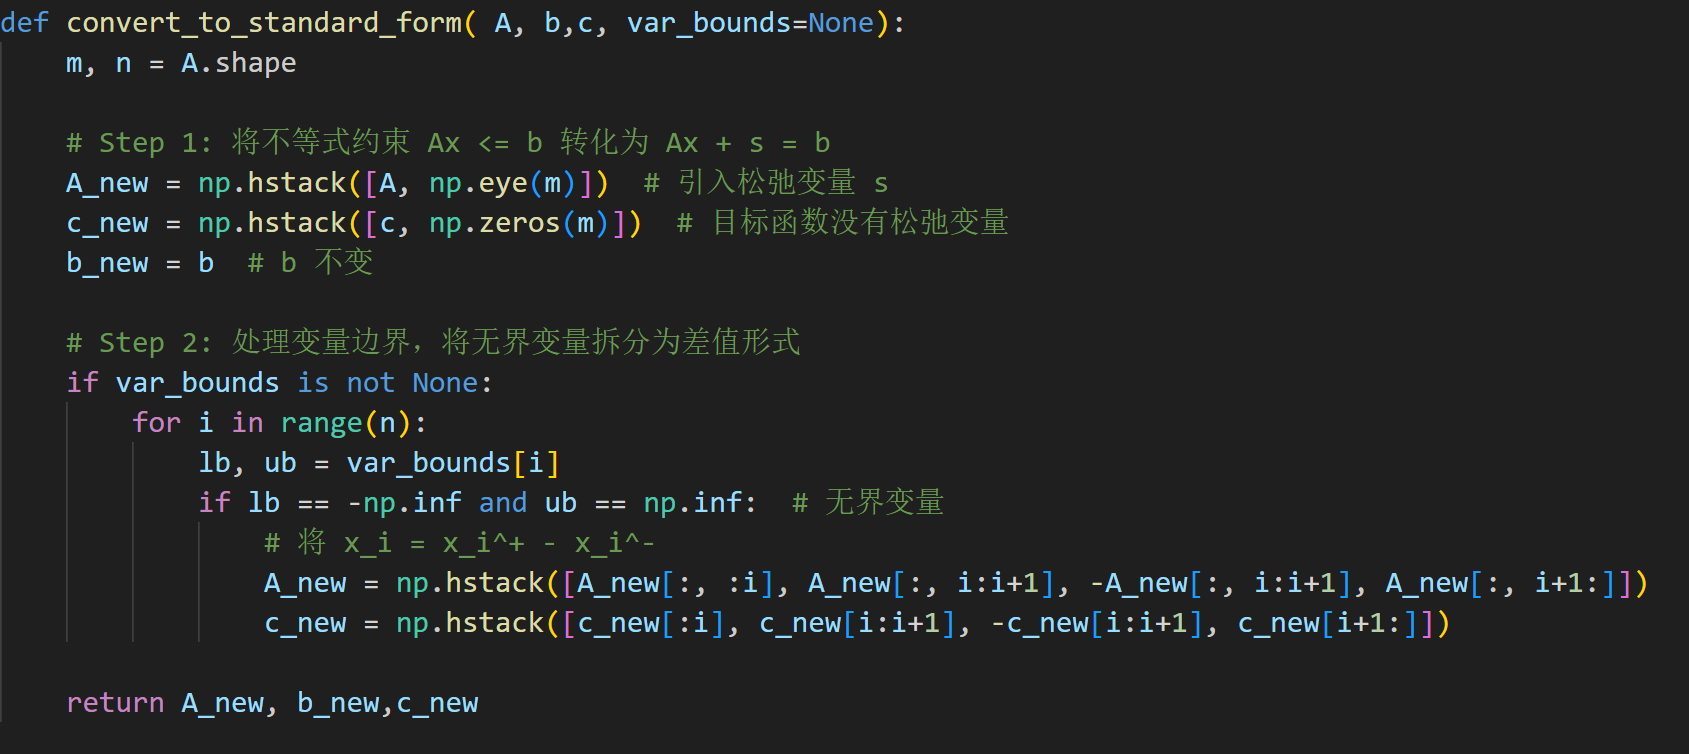
\includegraphics[width=0.8\textwidth]{屏幕截图 2024-11-05 104535.png}
\end{figure}

线性规划问题的一般形式为:
\[
\text{Maximize } \mathbf{c}^T \mathbf{x}
\]
subject to
\[
\mathbf{A} \mathbf{x} \leq \mathbf{b}, \quad \mathbf{x} \geq 0
\]
在实际应用中,约束条件往往是以不等式形式给出的,
需要将其转化为等式形式。通过引入松弛变量,
可以将不等式约束转化为等式约束,从而使问题能够
采用标准的单纯形法进行求解。

此外,线性规划问题中可能存在无界变量,为了
保证问题的求解稳定性,需要通过差分操作将无
界变量转化为有界变量。

\subsection{检查满秩}

\begin{figure}[H]
    \centering
    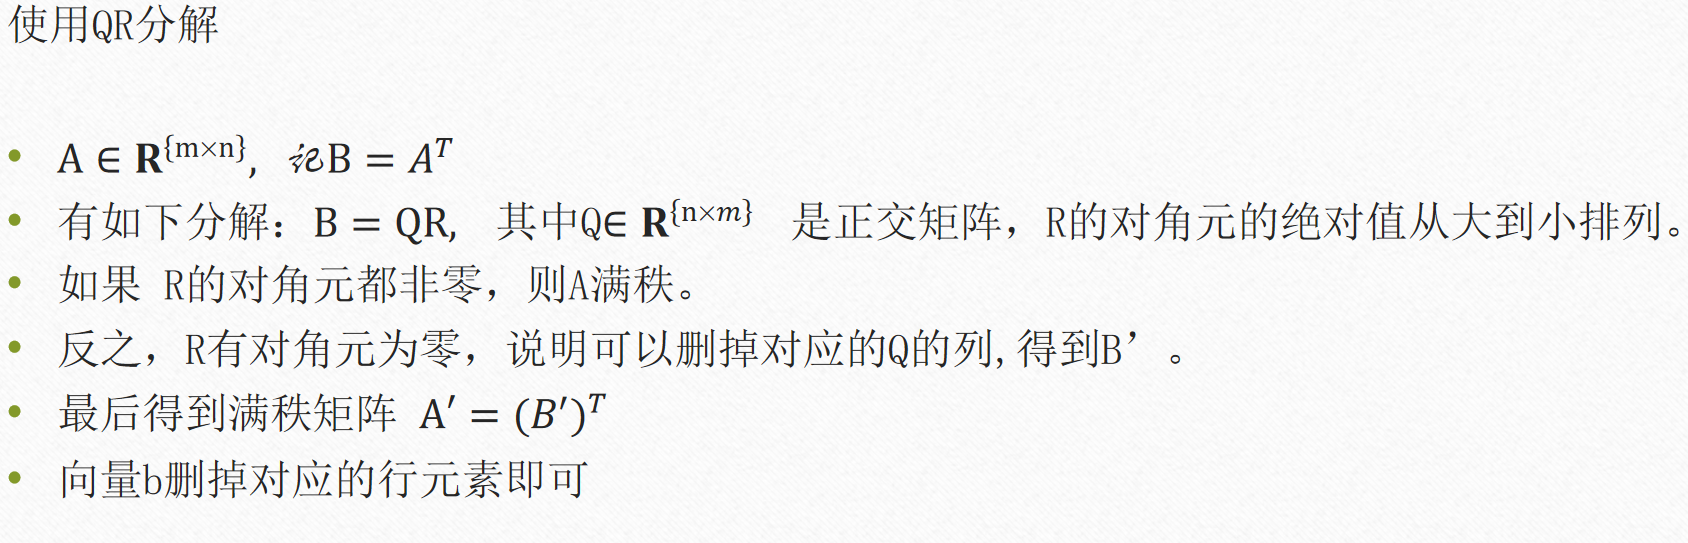
\includegraphics[width=0.8\textwidth]{屏幕截图 2024-11-05 111203.png}
\end{figure}

\begin{figure}[H]
    \centering
    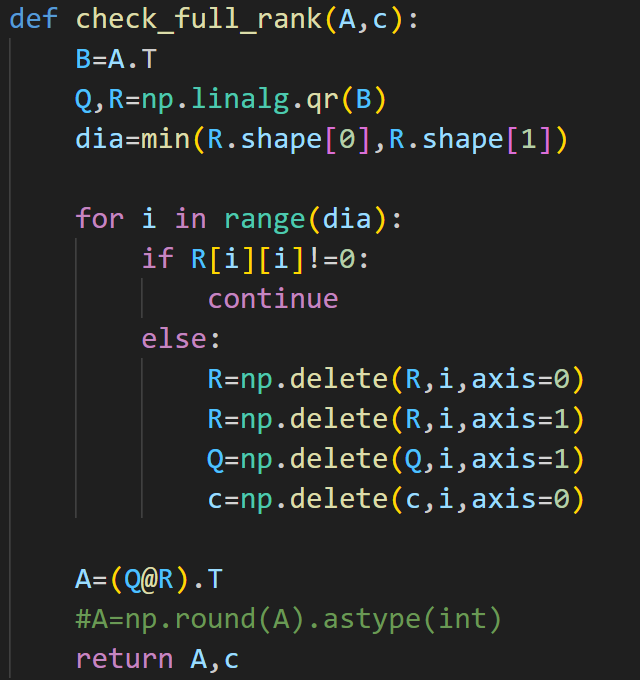
\includegraphics[width=0.6\textwidth]{屏幕截图 2024-11-05 104551.png}
\end{figure}

对于线性规划问题的约束矩阵 $\mathbf{A}$,我们需要检查其是否为
满秩矩阵。如果矩阵存在冗余约束或线性相关的约束,这会影响问
题求解的精度与稳定性。通过使用QR分解方法,可以检查矩阵是
否为满秩矩阵,并进行必要的转换,以确保算法在执行时的有效性。


\subsection{大M法获得初始可行基解}

\begin{figure}[H]
    \centering
    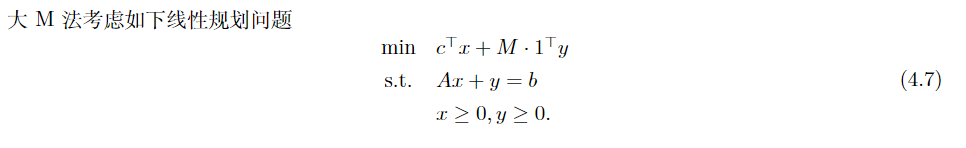
\includegraphics[width=0.8\textwidth]{屏幕截图 2024-11-05 111702.png}
\end{figure}

\begin{figure}[H]
    \centering
    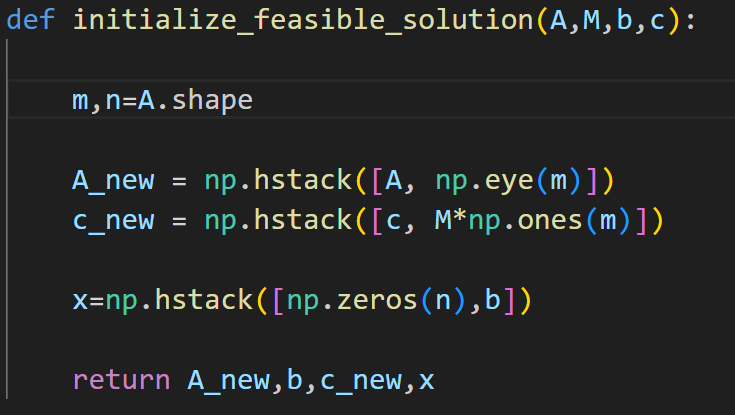
\includegraphics[width=0.8\textwidth]{屏幕截图 2024-11-05 104603.png}
\end{figure}

大M法是一种通过引入大数 M 以辅助求解初始可行解的方法。
通过对人工变量的引入和对大数的设置,我们可以使得线性规
划问题进入一个初始可行解。

\subsection{单纯形法}

\begin{figure}[H]
    \centering
    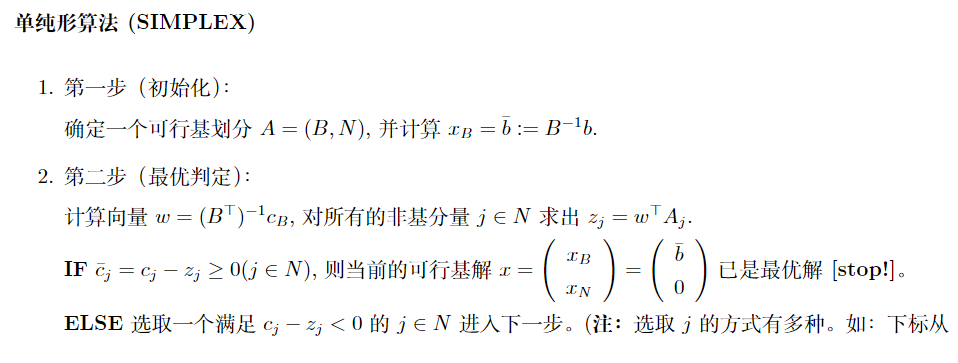
\includegraphics[width=0.8\textwidth]{屏幕截图 2024-11-05 112024.png}
\end{figure}

\begin{figure}[H]
    \centering
    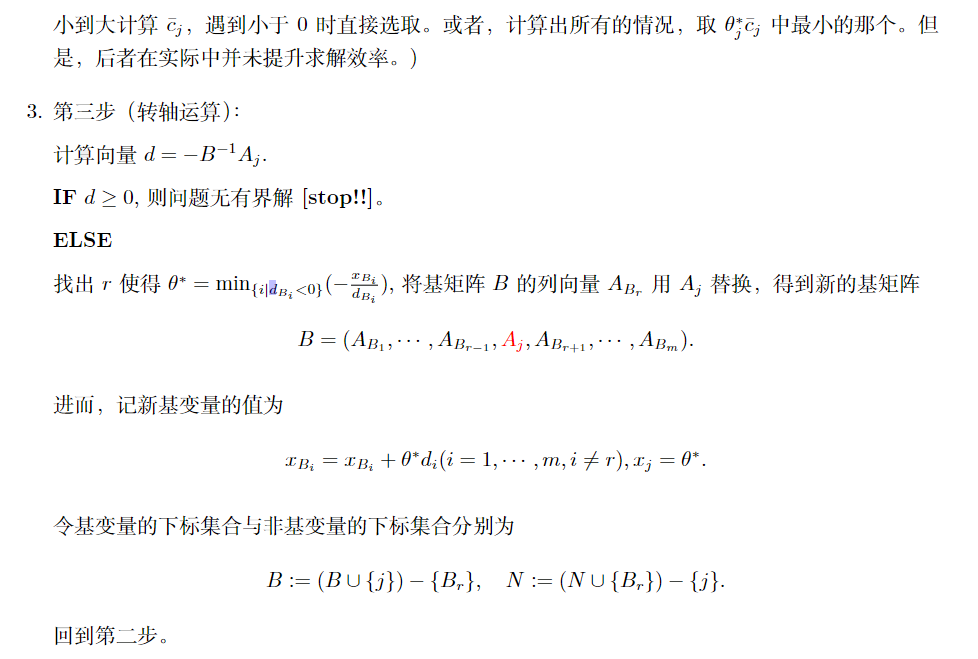
\includegraphics[width=0.8\textwidth]{屏幕截图 2024-11-05 112033.png}
\end{figure}

单纯形法是一种用于求解线性规划问题的常见算法,
通过迭代计算在约束条件下不断优化目标函数,直至
找到最优解。在本实验中,我们使用单纯形法进行求
解,并在迭代过程中采用**Bland’s Rule**避免出现循环情况。

\subsection{随机生成Abc}

\begin{figure}[H]
    \centering
    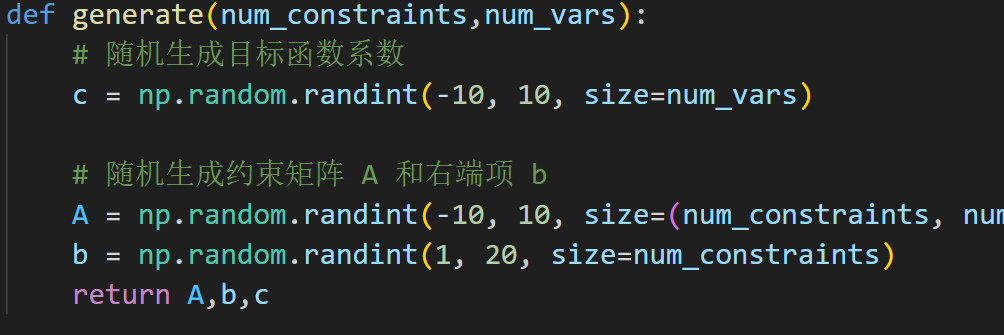
\includegraphics[width=0.8\textwidth]{屏幕截图 2024-11-05 110734.png}
\end{figure}

为了模拟实际应用中不同规模和结构的线性规划问题,
我们使用**random**函数生成随机矩阵 A、b 和 c,
并根据生成的随机矩阵求解线性规划问题。通过生成不
同规模和类型的矩阵,实验能够验证算法在不同情况下
的表现。

\section{实验结果}

\subsection{有可行解}

\begin{figure}[H]
    \centering
    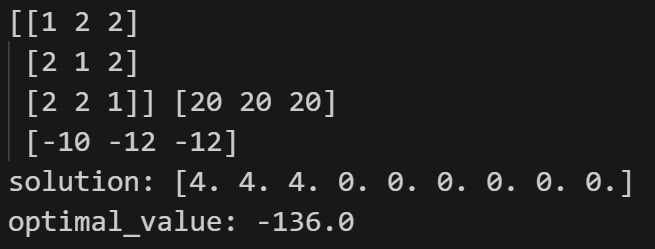
\includegraphics[width=0.6\textwidth]{屏幕截图 2024-11-05 114502.png}
\end{figure}

\subsection{有冗余秩}

\begin{figure}[H]
    \centering
    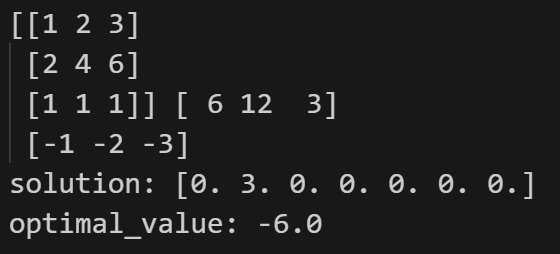
\includegraphics[width=0.6\textwidth]{屏幕截图 2024-11-05 114539.png}
\end{figure}

\subsection{无可行域}

\begin{figure}[H]
    \centering
    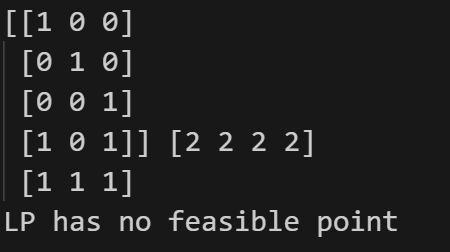
\includegraphics[width=0.6\textwidth]{屏幕截图 2024-11-05 114529.png}
\end{figure}

\subsection{无界}

\begin{figure}[H]
    \centering
    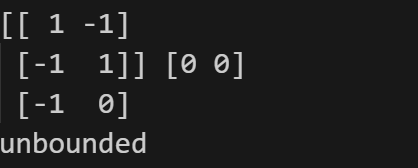
\includegraphics[width=0.6\textwidth]{屏幕截图 2024-11-05 114511.png}
\end{figure}

\subsection{随机生成}

\begin{figure}[H]
    \centering
    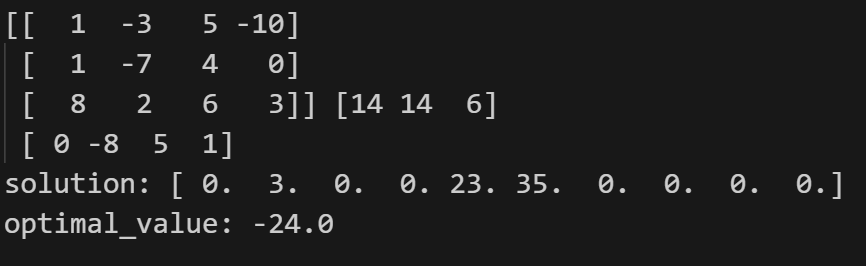
\includegraphics[width=0.6\textwidth]{屏幕截图 2024-11-05 114636.png}
\end{figure}

\begin{figure}[H]
    \centering
    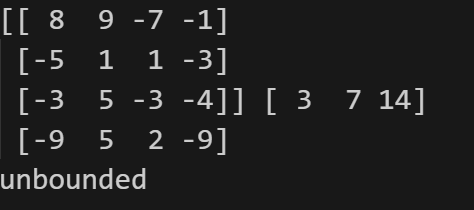
\includegraphics[width=0.6\textwidth]{屏幕截图 2024-11-05 114620.png}
\end{figure}

\begin{figure}[H]
    \centering
    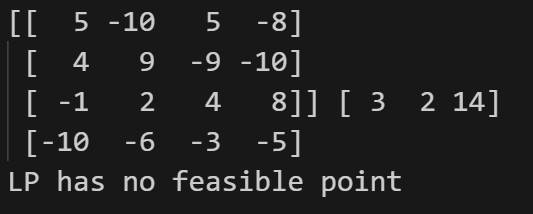
\includegraphics[width=0.6\textwidth]{屏幕截图 2024-11-05 114615.png}
\end{figure}

下面是运行时间随着规模增大的拟合图像。

以5为步长,从5依次计算到95,每种随机生成20组,仅统计有可行域的结果,
对运行时间求平均值和方差得到(纵轴单位为秒)。
\begin{figure}[H]
    \centering
    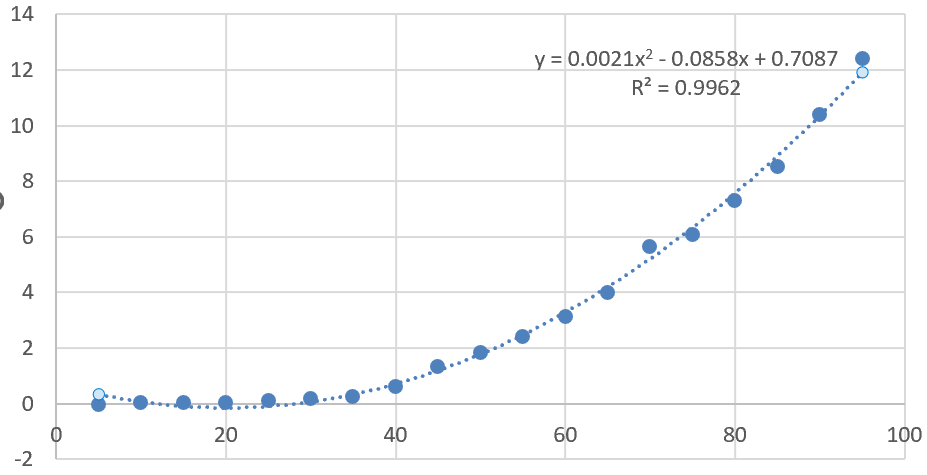
\includegraphics[width=0.8\textwidth]{屏幕截图 2024-11-05 150227.png}
	\caption{时间均值-阶数}
\end{figure}

\begin{figure}[H]
    \centering
    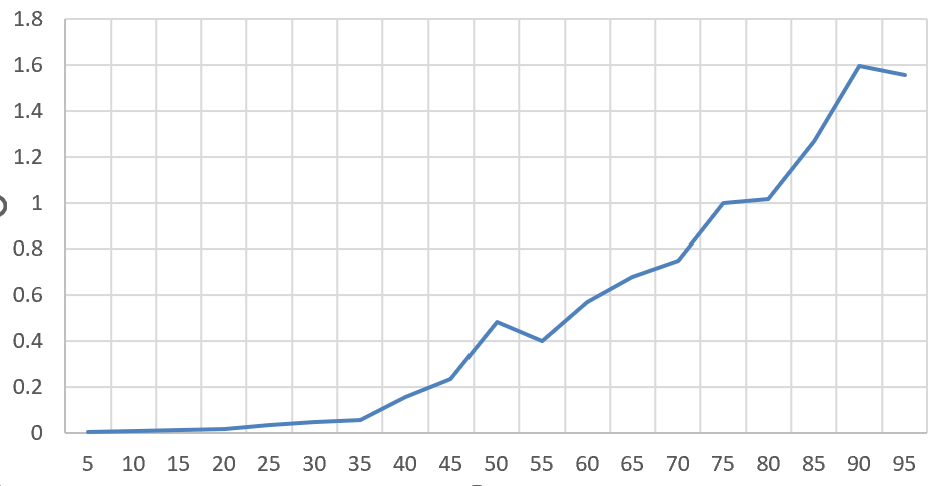
\includegraphics[width=0.8\textwidth]{屏幕截图 2024-12-03 112655.png}
	\caption{时间方差-阶数}
\end{figure}

可以发现,随着阶数规模的增加,求解时间也在增加,大致为二阶线性。标准差也在增加,且波动
明显大于平均时间。


\section{总结}

\begin{enumerate}
    \item 在 大M法 中,初始可行基解的选择非常关键。
    如果选择不当,可能会导致算法运行时间过长,甚至进
    入死循环。我们采用 Bland’s Rule 来避免循环,这是
    一个非常有效的策略。
    \item 矩阵规模与计算时间呈正相关(大致为二阶线性),随着矩阵规模的增大,
    计算时间显著增加,尤其是当约束条件较多时,计算时间增
    长更加明显。
    \item 大M法 和 单纯形法 是线性规划中常用的解法,对于
    小规模问题,两者的表现都较好。但随着规模的增加,求解
    时间较长时。
    \item 
    特殊情况的处理:在处理无可行解、无界解等特殊情况时
    ,实验系统能够及时反馈,并优化计算过程。
\end{enumerate}

\end{document}
